\chapter{Introduction}


\section{Statement of Aims} 

This body of work is concerned with \textit{inverse problems} \citep{Tarantola2005,Aster2013,Menke2012,Kaipio2006,Biegler2010,Idier2013}, also referred to as parameter inference or parameter estimation problems \citep{Box1973,Sprott2008,Casella1993,Cox2007}. Parameter inference based on observable data is a pursuit which transcends scientific disciplines. For geophysics, it is the most important method which allows data to be transformed from surface observations into subsurface images. The effectiveness of traditional methods of geophysical parameter inference is limited when characterizing non-linear systems with trade-offs between parameters and inherit non-uniqueness. Under these conditions probabilistic parameter inference has demonstrated utility in imaging the subsurface \citep{Tarantola2005}. With that in mind, this project seeks to explore the geophysical applicability of a recently developed method of probabilistic parameter inference, known as \underline{A}pproximate \underline{B}ayesian \underline{C}omputation (ABC), which has emerged from applied challenges in genetics \citep{Tavare1997,Beaumont2002,Sunnaker2013}. This project was started on January 5th, 2018 and concluded with the submission of this document on the 14th of October, 2018. All codes used in this project are written by the author and available at \url{https://github.com/tomconnell/abc-toy-problems} and \url{https://github.com/tomconnell/approximate-bayesian-tomography}.

\section{Parameter inference}

Parameter inference is the definition of unknown parameters, $\bm{\theta} = \{\theta_1,...,\theta_N\}$, for a causative model, $\mathcal{M}$, based on observed data, $\bm{y} = \{y_1,...,y_M\}$. For geophysics, we are interested in defining the physical properties of the subsurface (e.g. seismic velocity, density) from experimental data observed at the surface (e.g. seismic signals, gravitational acceleration). This search is alternatively referred to as the \textit{inverse problem} \citep{Tarantola2005,Aster2013,Menke2012}: 
\begin{equation}
\text{The inverse problem:}\ \bm{y} \rightarrow \bm{\theta}
\label{inverse_problem}
\end{equation}
Solving the inverse problem relies on the definition of deterministic physical models which link a parameterized subsurface model to simulated data., giving rise to the \textit{forward problem}:
\begin{equation}
\text{The forward problem:}\ \bm{\theta'} \rightarrow \bm{y'}
\label{forward_problem}
\end{equation}
The relationship between model parameters and resulting simulated data may be highly non-linear and is represented through the operator $\bm{g}$:
\begin{equation}
\bm{y} = \bm{g}(\bm{\theta})
\label{basic_data_parameters}
\end{equation}

%For geophysics, the unknown parameters, $\bm{\theta} = \{\theta_1,...,\theta_N\}$, for a causative model, $\mathcal{M}$, are sought based on observed data, $\bm{y} = \{y_1,...,y_M\}$. The relationship between model parameters and data may be highly non-linear and is represented through the operator $\bm{g}$:
%\begin{equation}
%\bm{y} = \bm{g}(\bm{\theta})
%\label{basic_data_parameters}
%\end{equation}
%Here we are interested in defining the physical properties of the subsurface (e.g. seismic velocity, density) from experimental data, $\bm{y}$, observed at the surface (e.g. seismic signals, gravitational acceleration). 
%Deterministic physical models, $\mathcal{M}$, link a parameterized subsurface model to simulated data, $\bm{y'}$. Imaging the subsurface collapses to a parameter inference problem \citep[p.1-2]{Tarantola2005}.\par

%Geophysical parameter inference belongs to a large class of problems known as \textit{inverse problems} \citep{Tarantola2005,Aster2013,Menke2012}. These methods use experimental data, $\bm{y}$, to infer the causative model parameters, $\bm{\theta}$. This contrasts with the \textit{forward problem}, which starts with a given set of model parameters, $\bm{\theta'}$, and produce a set of simulated data, $\bm{y'}$. Both areas are subject to considerable research and development. Of particular relevance to us is that the ability to solve the forward problem is required to solve the inverse problem.
%\begin{equation}
%\text{The inverse problem:}\ \bm{y} \rightarrow \bm{\theta}
%\label{inverse_problem}
%\end{equation}
%\begin{equation}
%\text{The forward problem:}\ \bm{\theta'} \rightarrow \bm{y'}
%\label{forward_problem}
%\end{equation}

\section{Probabilistic formulation}

Geophysical inverse problems come with a unique set of challenges. Often the experimental data has significant levels of uncertainty, the number of unknown model parameters may far exceed the amount of constraining data and the uncertainty in the physical model (the forward problem) may itself be large. These conditions weaken  traditional methods of parameter estimation.\par

Bayes' theorem, equation \ref{bayes}, is the basis for a probabilistic formulation to geophysical inverse problems \citep{Tarantola1982a,Mosegaard1995,Sambridge2002,Mosegaard2002,Tarantola2005}. The Bayesian formulation can quantify the uncertainty in the data and forward problem, scrutinize model non-uniqueness and constrain the solution with information obtained independent of the observed data. In this approach, geophysical inverse problems receive a full statistical treatment of uncertainty. The Bayesian method is fundamentally about embracing uncertainty and making use of all available information to update our state of knowledge. Bayes' theorem relies on the notion of conditional probability, i.e. $p(a|b)$ is the conditional probability of $a$ given event $b$ has occurred. Bayes' theorem is used to define the solution to the inverse problem as the PDF of the model parameters $\bm{\theta}$ conditioned on the observed data $\bm{y}$, $p(\bm{\theta}|\bm{y})$. This PDF is referred to as the \textit{posterior}:
\begin{equation}
p(\bm{\theta}|\bm{y}) = \frac{p(\bm{\theta}) p(\bm{y}|\bm{\theta})}{p(\bm{y})}
\label{bayes}
\end{equation}
Equation \ref{bayes} states that the prior distribution, $p(\bm{\theta})$, multiplied by $p(\bm{y}|\bm{\theta})$, over a normalization constant, $p(\bm{y})$, is equal to the posterior PDF, $p(\bm{\theta}|\bm{y})$.\par

The prior, $p(\bm{\theta})$, is a user-defined probability distribution which incorporates what is already known about the model parameters, $\bm{\theta}$, independent of the experimental data, $\bm{y}$. When trying to understand subsurface structure with surface data there may be prior knowledge. For example, the thickness of layers in a vertical stack may be known to be distributed according to a exponential probability distribution \citep{Mosegaard1995}. \par

Once data $\bm{y}$ is observed, $p(\bm{y}|\bm{\theta})$ can be regarded as a function of $\bm{\theta}$ rather than $\bm{y}$ (now fixed) and therefore it describes the likelihood of $\bm{\theta}$ given $\bm{y}$. If for two possible sets of model parameters $\bm{\theta_1}$ and $\bm{\theta_2}$ we have $p(\bm{y}|\bm{\theta_1}) > p(\bm{y}|\bm{\theta_2})$ then $\bm{y}$ is more likely to occur under $\bm{\theta_1}$ than $\bm{\theta_2}$. In this case, $p(\bm{y}|\bm{\theta})$ is called the \textit{likelihood} and commonly represented as $\mathcal{L}(\bm{\theta}|\bm{y})$. The likelihood is a central part of this thesis and is expanded upon in the next section.\par

The normalization constant $p(\bm{y}) = \int p(\bm{\theta}) p(\bm{y}|\bm{\theta})\ \text{d}\bm{\theta}$ is difficult to calculate and generally unconsidered. Statistics about the posterior such as maximum posterior value, mean, and standard deviation can still be computed from an unnormalized posterior density. The consequence of leaving $p(\bm{y})$ unevaluated is simply that single point values of the posterior have no probabilistic interpretation. Instead relative values must be evaluated where ratios cancel the normalization constant. Hence, Bayes' theorem is practically applied in the form:
\begin{equation}
p(\bm{\theta}|\bm{y}) \propto p(\bm{\theta}) p(\bm{y}|\bm{\theta})
\label{applied_bayes}	
\end{equation}
The posterior distribution, $p(\bm{\theta}|\bm{y})$, is the solution to a probabilistic formulation of an inverse problem. It is the complete state of knowledge about $\bm{\theta}$ given $\bm{y}$. Complete as it incorporates both what is already known, $p(\bm{\theta})$, as well as new experimental data, $\bm{y}$, through the likelihood. The probabilistic solution offers a philosophical shift compared to traditional solutions. A probability distribution over all model parameters is recovered offering in-built quantification of uncertainty, instead of a single `optimal' set of model parameters. \par

The probabilistic solution to inverse problems outlined above has been successfully applied e.g. to seismic tomography (e.g. \citet{Sambridge1999,Shapiro2002,Trampert2004,Khan2011}) and in joint inversions of geophysical data (e.g. \citet{khan2007joint,Moorkamp2010,Bodin2012,Shen2012,afonso2013a,afonso2013b,afonso2016}). Yet, for non-trivial problems there is no analytical solution for the posterior. A popular approach is to approximate the posterior via stochastic sampling, such as Monte Carlo or Markov chain Monte Carlo (MCMC). For subsurface models with many unknown model parameters, such as a 3D high-resolution grid, and where each posterior sample requires computationally expensive simulation from a deterministic physical model, highly efficient numerical sampling methods are required if the posterior is to be adequately defined within the current computational limits. \par



%The logic and strength of inversions with more than one dataset is that datasets with complimentary constraints on the same underlying model parameter space can minimize the range of acceptable models relative to their individual inversion. One example of this is a joint-inversion of surface wave dispersion curves, which  provide smooth continuous sensitivity to shear wave velocity, and receiver functions, which provide a sensitivity to the shear wave velocity discontinuities \citep{Bodin2012,Shen2012}. This advance is important as it overcomes the weakness of inversions when a single dataset cannot constrain a solution due to its large uncertainties or inherit non-uniqueness. The result has been more informed inference driving a more accurate understanding of the Earth.

\section{The likelihood}

%The likelihood is central to both Bayesian and frequentest statistical parameter inference. Both specifications of the prior distribution and likelihood are at the heart of Bayesian inference, the probabilistic framework adopted here. In practice, due attention should be paid to both, as they both play central roles in the posterior, equation \ref{applied_bayes}. However, as will be introduced in depth later, Approximate Bayesian Computation diverges from traditional Bayesian inference by circumventing calculation of the likelihood, instead using an approximation to the likelihood. Given ABC will move away from its use, it is important to understand what the likelihood offered and how it functioned. A particularly important component is the assumptions made in constructing the likelihood. \par

The likelihood is used after $\bm{y}$ is available to describe the plausibility of $\bm{\theta}$. Given this role, the probability $p(\bm{y}|\bm{\theta})$ in Bayes' theorem, equation \ref{bayes}, is practically applied as a conditional probability given $\bm{y}$, for varying values of $\bm{\theta}$ \citep[p.10]{Box1973}. Following \citet{Fisher1922}, this is referred to as the likelihood and is commonly denoted $\mathcal{L}(\bm{\theta}|\bm{y})$. This maps out a distribution of relative plausibility over $\bm{\theta}$ in describing the observed data $\bm{y}$. The likelihood is not necessarily a PDF and hence point values do not have a probabilistic interpretation. Only through comparison of relative values does the likelihood gain meaning \citep[p.11]{Box1973}.\par

%The likelihood is used after $\bm{y}$ is available to describe the plausibility of $\bm{\theta}$. It is a function of the parameters $\bm{\theta}$ to the model $\mathcal{M}$, given observed data $\bm{y}$. Hence it is denoted $\mathcal{L}(\bm{\theta}|\bm{y})$. However, the plausibility of $\bm{\theta}$ given $\bm{y}$ is proportional to the PDF of $\bm{y}$ given $\bm{\theta}$. This gives us the paradoxical statement:
%\begin{equation}
%\mathcal{L}(\bm{\theta}|\bm{y}) \propto \pi(\bm{y}|\bm{\theta})
%\label{likelihood_def}
%\end{equation}
%However this is resolved by considering $\pi(\bm{y}|\bm{\theta})$ at the observed $\bm{y}$, hence fixed, for varying $\bm{\theta}$. This maps out a distribution of relative plausibility over $\bm{\theta}$. The likelihood is not necessarily a PDF and hence point values contain no inherent information. Only through comparison of relative values does the likelihood gain meaning.\par

A full derivation of the likelihood is given from first assumptions \hyperref[tf1]{Technical figure 1} to the final forms which are commonly featured in geophysical inversions \hyperref[tf1]{Technical figure 2}.\par

For physical sciences a given observed data point, $y_i$, is considered equal to simulated data from a parameterized deterministic model, $\bm{g}(\bm{\theta})$, with additive statistical uncertainty from both the measurement process, $e^{\mathcal{D}}_i$, and the modelization process, $e^{\mathcal{M}}_i$:
\begin{equation}
y_i = z_i + e^{\mathcal{D}}_i
\end{equation}
\begin{equation}
z_i = g_i(\bm{\theta}) + e^{\mathcal{M}}_i
\end{equation}
\begin{equation}
y_i = g_i(\bm{\theta}) + e^{\mathcal{M}}_i + e^{\mathcal{D}}_i
\end{equation}
For the case of estimating $\bm{\theta} = \{\theta_1,...,\theta_N\}$ given $\bm{y} = \{y_1,...,y_M\}$, if it is assumed that the nature of the statistical uncertainty of measurement and modelization is independent and identically distributed from a Gaussian distribution then the likelihood takes the form (c.f. \citet[p.91-92]{gregory2005bayesian}): 
\begin{equation}
\begin{split}
\mathcal{L}(\bm{\theta}|\bm{y}) &= p(\bm{y}|\bm{\theta}) = p(y_1,...,y_m|\bm{\theta})\\
&\propto  \text{exp}\bigg[\sum_{i = 1}^{M}\frac{-(y_i-g_i({\bm{\theta}}))^2}{2\big((\sigma^{\mathcal{M}}_i)^2+(\sigma^{\mathcal{D}}_i)^2\big)}\bigg]
\end{split}
\label{likelihood-1}
\end{equation}

% In case in need to include the above likelihood scaling
% (2\pi)^{M/2}\Big(\prod_{i = 1}^{M}\big((\sigma^{\mathcal{M}}_i)^2+(\sigma^{\mathcal{D}}_i)^2\big)^{1/2}\Big)\
Otherwise, if the uncertainty is Gaussian distributed but correlated, covariance matrices $C_{\mathcal{D}}$ and $C_{\mathcal{M}}$ are combined to quantify the total statistical uncertainty and define a likelihood (c.f. \citet[p.35-36]{Tarantola2005}):
\begin{equation}
\mathcal{L}(\bm{\theta}|\bm{y}) \propto \text{exp}\bigg[-\frac{1}{2}(\bm{y}-\bm{g}(\bm{\theta}))^T(C_{\mathcal{M}}+C_{\mathcal{D}})^{-1}(\bm{y}-\bm{g}(\bm{\theta}))\bigg]
\label{likelihood-2}
\end{equation}

If more complicated models for uncertainty are determined or assumed then access to Bayesian parameter inference may close entirely if no closed form expression for the likelihood can be derived. For example, if the data uncertainty is irreducible to a simple standard distribution and the modelization errors are systematic and mesh-dependent (not uncommon in geophysics), then making the same derivations as is done in \hyperref[tf1]{Technical figure 2} may not be possible. The problem would have an intractable likelihood. This issue is encountered in genetics, and lead to the development of the likelihood-free methods of Approximate Bayesian Computation. For example, the coalescent \citep{Marjoram2006} describes how gene variants are passed down from a common ancestor, where coalescent events are approximated by an exponential distribution. This model is then overprinted by mutations, described by a Poisson distribution. As the number of samples of DNA expanded, it was not possible to formulate a likelihood to describe the time to the most recent common ancestor given the DNA set.\par

\newpage
\begin{tcolorbox}[enhanced jigsaw,breakable,pad at break*=1mm,title=Technical figure 1: General likelihood derivation, title filled,fonttitle=\sffamily\bfseries,fontupper=\sffamily\scriptsize,before upper={\parindent15pt}]
%\chapter{Box 1: Likelihood derivation}
\label{tf1}

\begin{multicols}{2}
\noindent \citet[p.89-90]{gregory2005bayesian} outline constructing a likelihood, $\mathcal{L}(\bm{\theta}|\bm{y})$, from starting assumptions. Firstly, a model for the data is assumed:
\begin{equation}
y_i = z_i + e_i
\label{general_form_inference}
\end{equation}
where $e_i$ is the uncertainty in the data, and $z_i$ is the data from the deterministic forward relation:
\begin{equation}
z_i = g_i(\bm{\theta})
\end{equation}
Both $z_i$ and $e_i$ are represented by distributions:
\begin{equation}
p(z_i|\bm{\theta}) = f_Z(z_i)
\label{fz_dist}
\end{equation}
\begin{equation}
p(e_i|\bm{\theta}) = f_E(e_i)
\label{fe_dist}
\end{equation}
We are interested in arriving in an equation for $p(y_i|\bm{\theta})$, which will define $\mathcal{L}(\bm{\theta}|\bm{y})$. However, the relationship in equation \ref{general_form_inference} specifies, $y_i$ depends on both $z_i$ and $e_i$. Hence, to arrive at $p(y_i|\bm{\theta})$ we must consider the distributions of equations \ref{fz_dist} \& \ref{fe_dist}. If we first consider the joint distribution $p(y_i,z_i,e_i|\bm{\theta})$ then our likelihood can be found by integrating out, 'marginalizing', $p(z_i|\bm{\theta})$ and $p(e_i|\bm{\theta})$ to leave a distribution for $p(y_i|\bm{\theta})$:
\begin{equation}
p(y_i|\bm{\theta}) = \int \int \text{d}z_i\ \text{d}e_i\ p(y_i,z_i,e_i|\bm{\theta})
\label{most_general_L}
\end{equation}
The definition of conditional probability allows equation \ref{most_general_L} to be rewritten as:
\begin{equation}
p(y_i|\bm{\theta}) = \int \int \text{d}z_i\ \text{d}e_i\ p(z_i,e_i|\bm{\theta})\ p(y_i|z_i,e_i,\bm{\theta})
\end{equation}
If we assume $z_i$ and $e_i$ are independent:
\begin{equation}
p(y_i|\bm{\theta}) = \int \int \text{d}z_i\ \text{d}e_i\ p(z_i|\bm{\theta})\ p(e_i|\bm{\theta})\ p(y_i|z_i,e_i,\bm{\theta})
\label{halfway_through_derivation}
\end{equation}
From the relationship in equation \ref{general_form_inference}, $y_i-z_i-e_i = 0$, $p(y_i|z_i,e_i,\bm{\theta})$ can be reasonably represented as a dirac-delta function such that:
\begin{equation}
p(y_i|z_i,e_i,\bm{\theta}) = \delta(y_i-z_i-e_i)
\label{dirac_equality}
\end{equation}
This is a natural definition, as the probability density of $y_i$ given $z_i$ and $e_i$ should be focused when the exact relation of equation \ref{general_form_inference} is met. The dirac-delta function serves this role perfectly while still exhibiting properties of a PDF, non-negative and $\int_{-\infty}^{\infty}\delta = 1$. Considering equation \ref{dirac_equality}, equation \ref{halfway_through_derivation} becomes:
\begin{equation}
p(y_i|\bm{\theta}) = \int \int \text{d}z_i\ \text{d}e_i\ p(z_i|\bm{\theta})\ p(e_i|\bm{\theta})\ \delta(y_i-z_i-e_i)
\end{equation}
Adopting the form from equations \ref{fz_dist} \& \ref{fe_dist}:
\begin{equation}
p(y_i|\bm{\theta}) = \int \text{d}z_i\ f_Z(z_i) \int \text{d}e_i\ f_E(e_i) \delta(y_i-z_i-e_i)
\label{almost_general_form}
\end{equation}
The dirac-delta function in the second integral of equation \ref{almost_general_form} serves to isolate the value/values of $f_E(e_i)$ when $e_i = y_i - z_i$. Hence, it is equivalent to consider:
\begin{equation}
\int \text{d}e_i\ f_E(e_i) \delta(y_i-z_i-e_i) = f_E(y_i - z_i)
\end{equation}
This leaves a general form for the likelihood $p(y_i|\bm{\theta})$ as: 
\begin{equation}
p(y_i|\bm{\theta}) = \mathcal{L}(\bm{\theta}|y_i) = \int \text{d}z_i\ f_Z(z_i)\ f_E(y_i - z_i)
\label{general_likelihood}
\end{equation}
However this general equation is not in a form which can be practically applied to inference problems. To achieve a practical form further assumptions must be made about the distributions $f_Z(z_i)$ and $f_E(e)$. This is done by assigning parametric distributions. As we will see in the next section, assigning Gaussian distributions will allow \ref{general_likelihood} to form a usable expression which will be our applied-form likelihood.
\end{multicols}
\end{tcolorbox}

The accurate calculation of equation \ref{likelihood-1} and equation \ref{likelihood-2} is an important aspect of running algorithms which sample the posterior distribution. Often likelihood values can be extremely small, to the point where they approach and cross the limits of floating point arithmetic (arithmetic underflow). Crossing this limit would lead to a divergence from posterior sampling due to erroneous Monte Carlo or MCMC algorithm steps. \hyperref[tf3]{Technical figure 3} expands on this topic. It covers the form in which the calculations take in order to be numerically stable.\par


\begin{tcolorbox}[enhanced jigsaw,breakable,pad at break*=1mm,title=Technical figure 2: Applied likelihood derivation, title filled,fonttitle=\sffamily\bfseries,fontupper=\sffamily\scriptsize,before upper={\parindent15pt}]
\label{tf2}
\begin{multicols}{2}
It is assumed that both $y_i$ and $z_i$ contain statistical uncertainty. For $y_i$ the source of statistical uncertainty is a result of the measurement process. While for $z_i$ the source of uncertainty is a result of modelization. It is necessary to distinguish between these two sources of uncertainty. The data uncertainty arising from the measurement process will be denoted $e^{\mathcal{D}}_i$, while modelization uncertainty will be denoted $e^{\mathcal{M}}_i$. As such:
\begin{equation}
y_i = z_i + e^{\mathcal{D}}_i
\end{equation}
\begin{equation}
z_i = \bm{g}(\bm{\theta}) + e^{\mathcal{M}}_i
\end{equation}
\begin{equation}
\therefore y_i = \bm{g}(\bm{\theta}) + e^{\mathcal{M}}_i + e^{\mathcal{D}}_i
\end{equation}
$e^{\mathcal{M}}_i$ and $e^{\mathcal{D}}_i$ are assumed to be uncorrelated. If it is assumed that $e^{\mathcal{D}}_i$ is described as independent and identically distributed from a Gaussian with a predetermined standard deviation $\sigma^{\mathcal{M}}_i$: 
\begin{equation}
p(z_i|\bm{\theta}) = f_Z(z_i) = \frac{1}{\sqrt{2\pi(\sigma^{\mathcal{M}}_i)^2}}\ \text{exp}\bigg[\frac{-(e^{\mathcal{M}}_i)^2}{2(\sigma^{\mathcal{M}\ 2}_i)^2} \bigg]
\end{equation} 
Likewise, if $e^{\mathcal{D}}_i$ is assumed to be i.i.d from a Gaussian with standard deviation $\sigma^{\mathcal{D}}_i$ then:
\begin{equation}
p(e_i|\bm{\theta}) = f_E(e_i) = f_E(y_i-z_i) = \frac{1}{\sqrt{2\pi(\sigma^{\mathcal{D}}_i)^2}}\ \text{exp}\bigg[\frac{-(e^{\mathcal{D}}_i)^2}{2(\sigma^{\mathcal{D}}_i)^2} \bigg]
\end{equation}
As a result of defining parametric distributions for $f_Z(z_i)$ and $f_E(y_i-z_i)$ the general definition of $\mathcal{L}(\bm{\theta}|y_i)$, equation \ref{general_likelihood}, can be evaluated. This is the convolution of the two distributions: 
\begin{equation}
\begin{split}
\mathcal{L}(\bm{\theta}|y_i) = \frac{1}{\sqrt{2\pi}\sqrt{(\sigma^{\mathcal{M}}_i)^2+(\sigma^{\mathcal{D}}_i)^2}}\\
\text{exp}\bigg[\frac{-(y_i-\bm{g}(\bm{\theta}))^2}{2\big((\sigma^{\mathcal{M}}_i)^2+(\sigma^{\mathcal{D}}_i)^2\big)}\bigg]
\end{split}
\label{single-data-likelihood}
\end{equation}\par

It should be noted that many "assumptions" here are in fact scientifically testable hypotheses. For example, given a measurement process/instrument it should be possible to determine the statistical properties uncertainty, such as how closely it conforms to a Gaussian and whether they are true i.i.d samples or correlated in some manner. Likewise, the same can be done for modelization uncertainty. One scheme to classify the statistical properties, standard deviation and covariance matrix, of modelization uncertainty in the parameterization of geophysical forward problems is outlined in \citet{afonso2013b}.\par

Equation \ref{single-data-likelihood} defines the likelihood for a single data point. How then to move forward with a full dataset?\par

If you have a set of data $\bm{y} = \{y_1,...,y_M\}$, where each $y_i$ term is independent then, considering uncertainty in the data and model as i.i.d Gaussian:
\begin{equation}
\begin{split}
p(\bm{y}|\bm{\theta}) &= p(y_1,...,y_m|\bm{\theta})\\
&= (2\pi)^{M/2}(\prod_{i = 1}^{M}\big((\sigma^{\mathcal{M}}_i)^2+(\sigma^{\mathcal{D}}_i)^2\big)^{1/2})\\ 
& \text{exp}\bigg[\sum_{i = 1}^{M}\frac{-(y_i-\bm{g}({\bm{\theta}}))^2}{2\big((\sigma^{\mathcal{M}}_i)^2+(\sigma^{\mathcal{D}}_i)^2\big)}\bigg]
\label{used-likelihood-1}
\end{split}
\end{equation}
Equation \ref{used-likelihood-1} is the likelihood $\mathcal{L}(\bm{\theta}|\bm{y})$ for i.i.d Gaussian uncertainty.\par

For the case of correlated Gaussian uncertainty vectors of data and model parameters can be represented by a multivariate Gaussian distributions, defined with covariance matrices $C_{\mathcal{D}}$ and $C_{\mathcal{M}}$ respectively, such that:
\begin{equation}
f_Z(z) \propto \text{exp}\bigg[-\frac{1}{2}(\bm{y}-\bm{g}(\bm{\theta}))^TC_{\mathcal{M}}^{-1}(\bm{y}-\bm{g}(\bm{\theta}))\bigg]
\end{equation}
\begin{equation}
f_E(e) \propto \text{exp}\bigg[-\frac{1}{2}(\bm{y}-\bm{g}(\bm{\theta}))^TC_{\mathcal{D}}^{-1}(\bm{y}-\bm{g}(\bm{\theta}))\bigg]
\end{equation}
Then the likelihood involves a combination of their covariance matrices:
\begin{equation}
\mathcal{L}(\bm{\theta}|\bm{y}) \propto \text{exp}\bigg[-\frac{1}{2}(\bm{y}-\bm{g}(\bm{\theta}))^T(C_{\mathcal{M}}+C_{\mathcal{D}})^{-1}(\bm{y}-\bm{g}(\bm{\theta}))\bigg]
\label{used-likelihood-2}
\end{equation}
Equation \ref{used-likelihood-1} and \ref{used-likelihood-2} represent commonly implemented forms of the likelihood. It is instructive to understand the origin of the likelihood function as often it is overlooked in applied studies. Of particular importance are the explicit assumptions which are necessary steps in construction. Assumptions include:
\begin{enumerate}
\item The form of the model, equation \ref{general_form_inference}
\item The i.i.d Gaussian nature of measurement and modelization statistical uncertainty, or
\item The correlated multivariate Gaussian nature of the measurement and modelization uncertainty
\end{enumerate}
A shift away from these assumptions is likely to close access to a likelihood function.
\end{multicols}
\end{tcolorbox}

The likelihood for a single dataset can be built upon to form a joint likelihood. As long as the two datasets are independent then equations \ref{likelihood-1} and \ref{likelihood-2} can be expanded for two datasets, here $\bm{y}^a$ and $\bm{y}^b$. Consider the joint form of equation \ref{likelihood-2}:
\begin{multline}
\mathcal{L}(\bm{\theta}|\bm{y}^a,\bm{y}^b) = \mathcal{L}(\bm{\theta}|\bm{y}^a)\ \mathcal{L}(\bm{\theta}|\bm{y}^b)
\propto \text{exp}\bigg[-\frac{1}{2}(\bm{y}^a-\bm{g}^a(\bm{\theta}))^T(C_{\mathcal{M}^a}+C_{\mathcal{D}^a})^{-1}(\bm{y}^a-\bm{g}^a(\bm{\theta}))\bigg]\ \\
\text{exp}\bigg[-\frac{1}{2}(\bm{y}^b-\bm{g}^b(\bm{\theta}))^T(C_{\mathcal{M}^b}+C_{\mathcal{D}^b})^{-1}(\bm{y}^b-\bm{g}^b(\bm{\theta}))\bigg]
\label{joint-likelihood}
\end{multline}
As a result of the different scale of various dataset residuals, $(\bm{y}-\bm{g}(\bm{\theta}))^T(C_{\mathcal{M}}+C_{\mathcal{D}})^{-1}(\bm{y}-\bm{g}(\bm{\theta}))$, the joint likelihood equation \ref{joint-likelihood} can be  dominated by a dataset with significantly more data points or larger residual values. This impact can also extend through to the prior, where a joint or single likelihood can overwhelm a prior. This problem called for a solution in the form of a weighting scheme to balance the input of the different datasets. Some common forms of weighting schemes for two datasets are:
\begin{equation}
\text{residual}^a, \frac{1}{c}\ \text{residual}^b
\end{equation}
\begin{equation}
c\ \text{residual}^a, 1-c\ \text{residual}^b
\end{equation}
where $c$ is the weighting factor to be defined. The most common scheme for defining the weighting factors is ad-hoc. It relies on running synthetic tests to determine when the solution is giving a balance between the two datasets. This approach is likely to be biased by our expectations of synthetic tests. The resulting parameter uncertainties may not truly reflect the uncertainty associated with the combination of the two complimentary datasets. \par

%At this stage this ad-hoc weighting is deemed necessary. There is no other obvious way to balance the impact each dataset has in the currently established likelihood framework. New methods in statistics, which circumvent evaluating the likelihood may offer improved statistical properties in light of the shortfalls in combining datasets with traditional likelihood machinery. \par

%The likelihood in its current form, mixes and dilutes the information about closeness and model performances into a single metric. While this is necessary for calculation of the M-H acceptance ratio, this may not be the best way to guide an inversion scheme. More aspects of the model can be leveraged to explore areas of the parameter space which are deemed important, and this can be fed from the residuals to the proposal distribution so as to avoid blind, wasteful updates in an inversion scheme. Simulated datasets give us a lot of information which can never be captured by a single metric of mixed residuals. As such, it may be very worthwhile trying to leverage the available information.\par

%Other disciplines have found Approximate Bayesian Computation offers an alternative to traditional likelihood machinery which can utilize more of what we know about the structure, physics and nature of the problems at hand. This is contrast to the simplifications which have been implicit in the construction of Bayesian inference and the form of the algorithms. Ideally we should be able to leverage the true complexity of the problem and the breadth of information we already know. In light of this goal Approximate Bayesian Computation is introduced in the next section.  

\pagebreak
\begin{tcolorbox}[enhanced jigsaw,breakable,pad at break*=1mm,title=Technical figure 3: Stable computation of likelihood values, title filled,fonttitle=\sffamily\bfseries,fontupper=\sffamily\scriptsize]
\label{tf3}

\begin{multicols}{2}

The stable computation of likelihood values is an essential component of running algorithms which resolve posterior distributions. This can be an issue as the value of the likelihood for a given set of parameters can be extraordinarily small, to the point where these values approach or cross the limits of what can be stored in a computers memory. \par

\indent Consider a unit hyper sphere that is located in a unit hyper cube. In low dimensions the sphere inside a cube takes up a large \% of the cubes volume. However, as the dimension increases this volume very rapidly diminishes. Figure \ref{hyper-objects} illustrates this relationship. The purpose of this example is to demonstrate that high dimensional spaces are very sparse. Geophysical inverse problems suffer particularly from this dimensionality, our images have many unknown parameters. Hence problems arising as a result of dimensionality, often referred to as \textit{the curse of dimensionality}, are of particular importance to geophysics. \par

\begin{figure}[H]
	\centering
	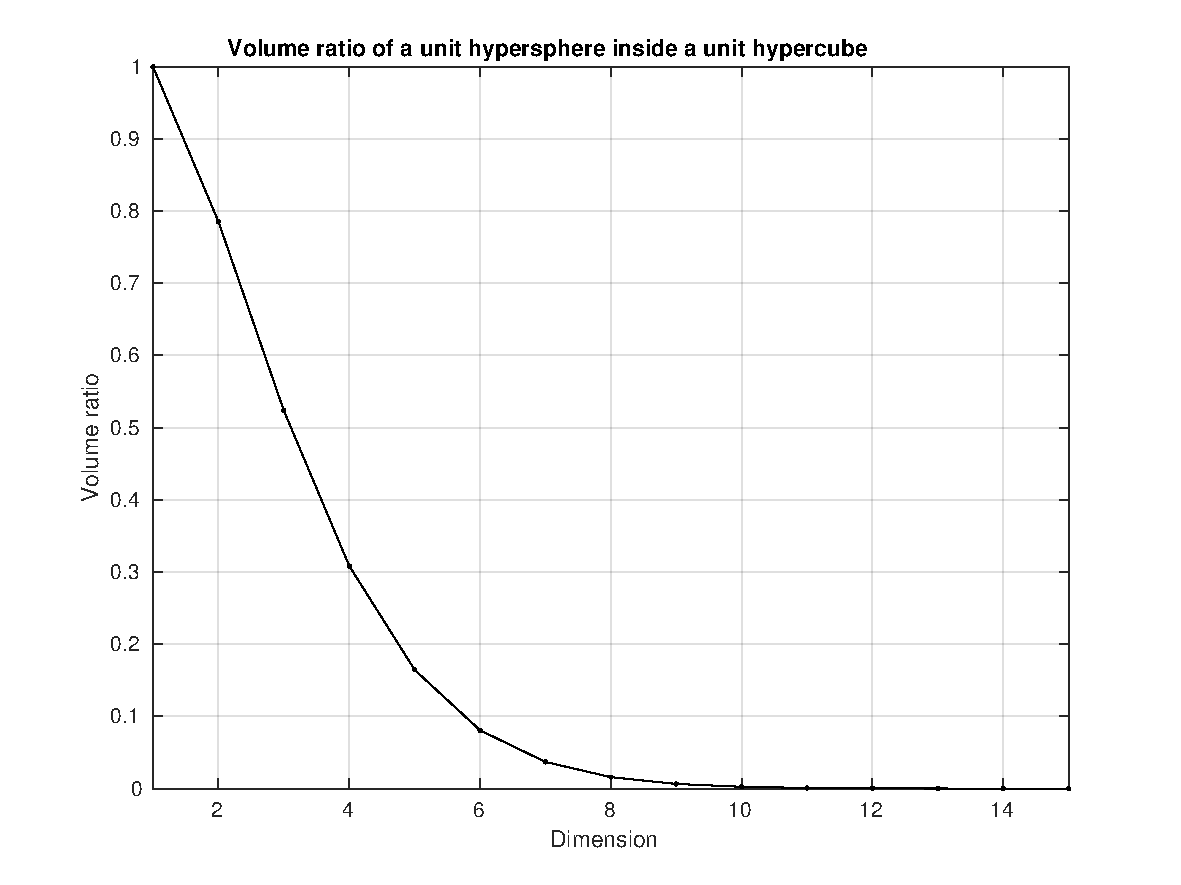
\includegraphics[scale=0.35]{hyperobjects.pdf}
	%\caption{The volume ratio of a unit hyper sphere, $2\pi^{d/2}r^d/d/\Gamma(d/2)$, inside a unit hyper cube, $(2r)^d$, as a function of dimension, $d$. This example is inspired by \citet{Laine2008}.}
	\label{hyper-objects}
\end{figure}

For a likelihood distribution over a sparse high dimensional space, the majority of the space will be extraordinarily empty - i.e. with very low probability. Considering probability is a value between 1 and 0, that means a lot of parameter space will have a likelihood very close to 0. Given this circumstance it is essential to be able to accurately compute and compare extremely small probability values. The risk of improper evaluation and comparison is erraneious steps in algorithms and a divergence from the posterior the algorithm is supposed to be sampling. In short your solution will be wrong. \par

\indent How to overcome this issue? The solution is to compute the natural logarithm of the likelihood. Figure \ref{nat-log} shows taking the natural logarithm of probability values. The result is very small probability values become very large negative numbers.

\begin{figure}[H]
	\centering
	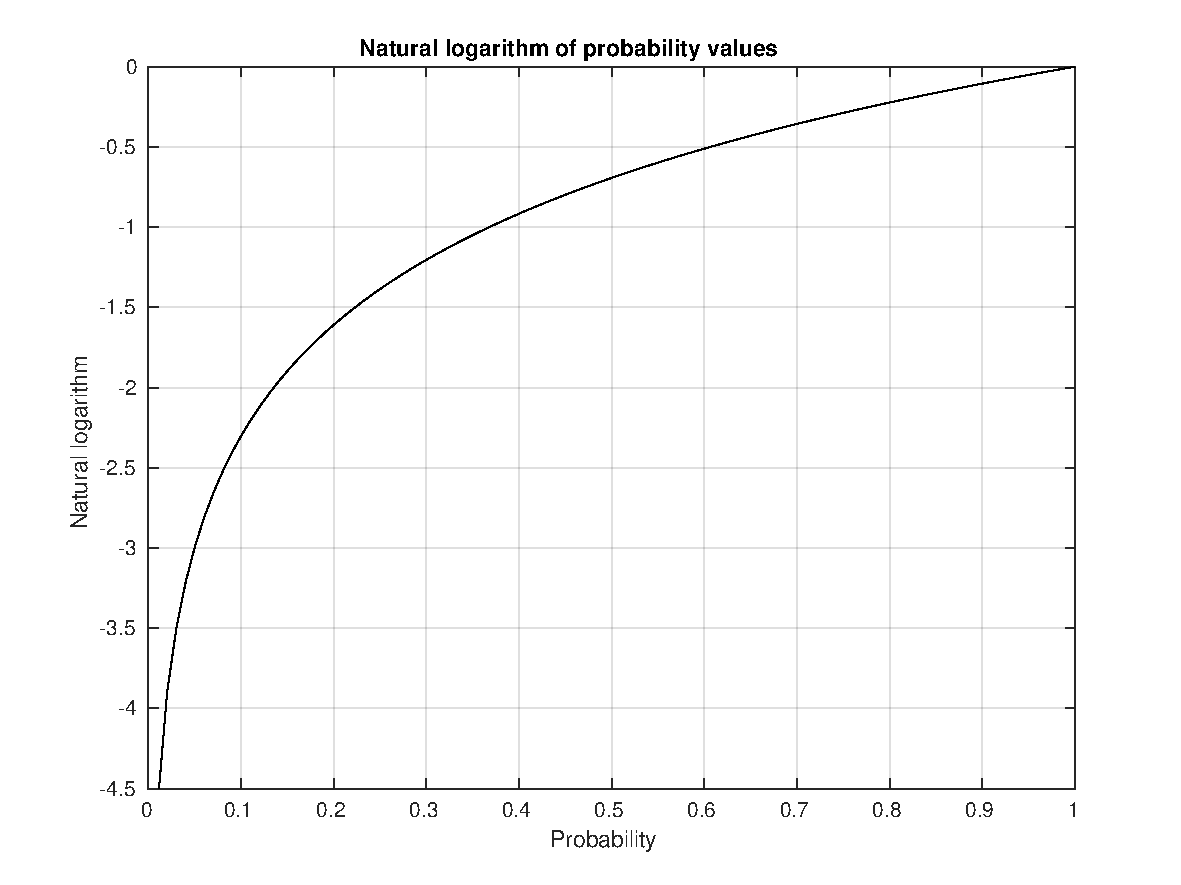
\includegraphics[scale=0.35]{nat-log.pdf}
	%\caption{The natural logarithm of probability values}
	\label{nat-log}
\end{figure}

These very large negative numbers transform a very small value, close to or crossing the limits of CPU memory, into a large number which can be easily stored. \par

\indent For a Gaussian likelihood, taking the natural logarithm of an unnormalized likelihood is in effect removing the exponential term. Consider the likelihood as in equation \ref{likelihood-2}. Repeated here
\begin{equation}
\mathcal{L}(\bm{\theta}|\bm{y}) \propto \text{exp}\bigg[-\frac{1}{2}(\bm{y}-\bm{g}(\bm{\theta}))^T(C_{\mathcal{M}}+C_{\mathcal{D}})^{-1}(\bm{y}-\bm{g}(\bm{\theta}))\bigg]
\label{repeat-likelihood-2}
\end{equation}
For $l(\bm{\theta}|\bm{y}) = \text{ln}(\mathcal{L}(\bm{\theta}|\bm{y}))$
\begin{equation}
l(\bm{\theta}|\bm{y}) \propto -\frac{1}{2}(\bm{y}-\bm{g}(\bm{\theta}))^T(C_{\mathcal{M}}+C_{\mathcal{D}})^{-1}(\bm{y}-\bm{g}(\bm{\theta}))
\label{log-likelihood}
\end{equation}
Reference to the negative log-likelihood would then mean
\begin{equation}
-l(\bm{\theta}|\bm{y}) \propto \frac{1}{2}(\bm{y}-\bm{g}(\bm{\theta}))^T(C_{\mathcal{M}}+C_{\mathcal{D}})^{-1}(\bm{y}-\bm{g}(\bm{\theta}))
\label{negative-log-likelihood}
\end{equation}

The negative log-likelihood is then a large positive number for very small probability values. Often minimization of an equation in the form of equation \ref{negative-log-likelihood} is the goal of linearized inversion schemes. Herein lies a connection between the likelihood function and linearized schemes, the result of a successful linearized inversion represents the minimum of the negative log-likelihood, $-l(\bm{\theta}|\bm{y})$. Which is also the maximum likelihood value. However our goal is generally broader. To explore the joint posterior distribution, a function of both likelihood and prior. This goal in high dimensional space necessitates Markov chain Monte Carlo (MCMC) sampling. So how does our shift to working with the natural logarithm of the likelihood impact this algorithm? \par

\indent For a MCMC algorithm with stationary distribution which is the posterior $p(\bm{\theta}|\bm{y})$, the key ingredient is evaluating the Metropolis-Hastings acceptance ratio, $\alpha$
\begin{equation}
\alpha = \frac{\mathcal{L}(\bm{\theta^*}|\bm{y})\ p(\bm{\theta^*})}{\mathcal{L}(\bm{\theta}|\bm{y})\ p(\bm{\theta})}
\label{acceptance-ratio}
\end{equation}
Where $^*$ represents a candidate move from the proposal distribution $q(\bm{\theta},.)$. As long as the proposal distribution is a symmetric distribution the ratio $q(\bm{\theta^*},\bm{\theta})/q(\bm{\theta},\bm{\theta^*})$ does not need to be computed as part of $\alpha$.\par

\indent Hence, the ratio of posterior values needs to be computed at each time step over the parameter space. The raw posterior values will be prone to numerical underflow due to the limits of CPU memory, hence the log values for the likelihood must be used in this calculation. How does the form of $\alpha$ get adjusted within a computer program to ensure stable and reliable computation?\par

\indent This shift represents a major divergence between how the theory is established in equation form, and the practical application in computer code.\par

\indent Consider we have access to the log-likelihood and log-prior. Recall the logarithm rules where $\text{ln}(xy) = \text{ln}(x)+\text{ln}(y)$ and $\text{ln}(x/y) = \text{ln}(x)-\text{ln}(y)$. Then
\begin{equation}
\alpha = \text{exp}\Big[\Big(l(\bm{\theta^*}|\bm{y})\ -\ l(\bm{\theta}|\bm{y})\Big)\ +\ \Big(\text{ln}\big(p(\bm{\theta^*})\big)\ -\ \text{ln}\big(p(\bm{\theta})\big)\Big)\Big]
\label{stable-acceptance-ratio}
\end{equation}
The resulting acceptance-ratio computed here will be equivalent to equation \ref{acceptance-ratio}, however, now the probability densities required in the computation will be restricted to large numbers, stable in their computation and comparison. The end result, a reliable MCMC algorithm.
\end{multicols}
\end{tcolorbox}
% Introduce issue which arises due to the different scale of the terms in this new Metropolis-Hastings acceptance ratio

%The shift of acceptance ratio from equation \ref{acceptance-ratio} to equation %\ref{stable-acceptance-ratio} introduces computational stability, however, a %new issue is introduced. The shift from products and ratios to addition and %subtraction means that the scales of the log-likelihoods and log-priors need %to be balanced. If one is much larger than the other then it will dominate the %calculation. This is true for calucluations of a one data set likelihood and %prior, as well as joint inversion schemes which introduce multiple individual %likelihoods into the calculation. The result has been the emergence of an ad-%hoc scaling regime for joint inversions. This directly counters the probematic %situation where the number of datapoints in the dataset leads to a %significantly different scaled log-likelihood. The standard form for joint %inversion likelihoods is given in equation XX. It can be seen that all dataset %are cobined to form a single joint log-likelihood. Two examples of scaling %schemes are
%\begin{equation}
%l_{joint} = l_1 + \frac{1}{c} l_2
%\end{equation}
%\begin{equation}
%l_{joint} = c l_1 + (1-c) l_2
%\end{equation}
%where $c$ is the scaling constant introduced. A similar scheme can be %introduced for 2+ datasets. The value of $c$ can then be set by repeated %inversion experiments which seek a known solution, the value can be taken by %what gives balanced solutions which utilise the information brought in by both %datasets.\\

%However, such a user defined weighting will be biased by our expectations in %synthetic tests. The final uncertainties may not accurately reflect the %uncertainty present in a real world problem. This may mean compromised %statistical properties the probabilitic Bayesian method guarentees to deliver.  %\\

%At this stage there is no "solution". A joint likelihood which utilises user %defined weights is currently the accepted system for joint inversion. But this %system should not be blindly accepted. Part of the scope of this thesis is %question the statistical underpinning of this form of the likelihood and probe %alternate formulations.


\section{Approximate Bayesian Computation}
\label{ApproximateBayesianComputation}

The likelihood, while underpinning a system which is formally strong and practically useful for geophysics, does suffer some weaknesses which are implicit in its construction and application. The likelihood limits the number of models (combined deterministic forward and uncertainty) which can be considered and applied as it requires a closed form expression. The likelihood also mixes and dilutes the available information about the data fit and model into a single metric. While necessary in the likelihood framework, this may not be the best way to drive an inversion scheme. Other disciplines have found Approximate Bayesian Computation offers an alternative to traditional likelihood machinery which can utilize more of what is known about the structure, physics and nature of the parameter inference problems at hand \citep{Tavare1997,Ratmann2009,vrugt2013toward}. It opens inference to a broader range of models and likewise offers formal statistical guarantees \citep{Sunnaker2013}.\par

Likelihood-free methods for Bayesian inference have been developed in response to parameter estimation problems where it is not possible to formulate or justify a closed form likelihood (e.g. \citet{Tavare1997,Fu1997,Weiss1998a,Pritchard1999a,Beaumont2002,Marjoram2003}). Instead, likelihood-free methods target the same posterior distribution without evaluating a likelihood. The algorithms and methods of likelihood-free Bayesian inference have been termed \textit{Approximate Bayesian Computation} (ABC). ABC simply requires the ability to simulate data given model parameters. Problems ripe for attack by ABC are common in science due to the breadth of models which have been developed to describe natural systems. It is frequently the case that the uncertainty associated with the data can be simulated rapidly but explicit formulas for probability distributions are difficult to formulate, expensive to evaluate, impossible to justify, or do not exist. Hence, traditional likelihood machinery becomes infeasible. ABC is a means to overcome these issues, it is backed by a sound theoretical underpinning and is subject to a rapidly expanding set of literature \citep{Ratmann2009,Blum2010,vrugt2013toward,Sunnaker2013,Blum2013,Sadegh2014,Pudlo2015,meeds2015hamiltonian,Lintusaari2016,gutmann2016bayesian,sisson2016handbook,Li2017}. \par

The premise of ABC begins with the notion that a set of model parameters, $\bm{\theta}$, is a sample from the posterior if the observed data, $\bm{y}$, and a simulated dataset, $\bm{y^*}$, are equal. Algorithm \ref{basicalg} generates i.i.d samples from the posterior $p(\bm{\theta}|\bm{y})$ (cf. \citet{Marjoram2003}).

\begin{algorithm}[H]
	\caption{ }
	\begin{algorithmic}
		\State 1. Generate $\bm{\theta^*}$ as a random sample from $p(\bm{\theta})$		
		\State 2. Simulate $\bm{y^*}$ from the forward operator $\bm{g_s}(\bm{\theta^*})$		
		\State 3. Accept $\bm{\theta^*}$ as a posterior sample if $\bm{y^*} = \bm{y}$		
		\State 4. Repeat
	\end{algorithmic}
	\label{basicalg}
\end{algorithm}

The operator $\bm{g_s}$ in Algorithm \ref{basicalg}, and all of likelihood-free inference, differs from the forward operators traditionally defined in geophysics. Forward operators in geophysics are \textit{deterministic}. That is, for a given set of model parameters, $\bm{\theta}$, the output of the forward operator $\bm{g}(\bm{\theta})$ will always be the same. The uncertainty in both data and model, are then later built into the construction of a likelihood. The ABC forward operator which simulates data, $\bm{g_s}$, is \textit{stochastic}. That is, the uncertainty from both data and modelization is built into the simulation process. As a result of this modification, algorithm \ref{basicalg} does not require the formulation or evaluation of a likelihood. The ABC forward operator $\bm{g_s}$ allows a practitioner to build in whatever uncertainty is justified for the scientific problem at hand. \par

Algorithm \ref{basicalg} is acceptable for basic problems where the datasets $\bm{y}$ and $\bm{y^*}$ are a discrete probability function, e.g. integers \citep{Tavare1997,Fu1997}. However, for large and continuous datasets the probability of generating a sample where the acceptance criteria, $\bm{y^*} = \bm{y}$, is met diminishes to levels unacceptable for parameter inference. ABC relaxes the problematic requirement of equality by accepting samples when the distance between $\bm{y^*}$ and $\bm{y}$, $\text{d}(\bm{y},\bm{y^*})$, is less than a tolerance value $\epsilon$ \citep{Weiss1998a}. This method, algorithm \ref{ABCfulldatatolerance}, does not target our true posterior of interest, but instead, the ABC posterior $p(\bm{\theta}|\text{d}(\bm{y},\bm{y^*})\leq\epsilon)$ which approximates the true posterior. 

\begin{algorithm}[H]
	\caption{ }
	\begin{algorithmic}
		\State 1. Generate $\bm{\theta^*}$ as a random sample from $p(\bm{\theta})$		
		\State 2. Simulate $\bm{y}$ from the forward operator $\bm{g_s}(\bm{\theta^*})$		
		\State 3. Accept $\bm{\theta^*}$ as a posterior sample if $\text{d}(\bm{y},\bm{y^*})\leq\epsilon$		
		\State 4. Repeat
	\end{algorithmic}
	\label{ABCfulldatatolerance}
\end{algorithm}

Algorithm \ref{ABCfulldatatolerance} requires a user specified metric, $\text{d}$, which defines the distance between datasets. Common choices are the absolute-value norm, Euclidean distance and Mahalanobis distance. Likewise, the value for the tolerance $\epsilon$ must be user specified. As $\epsilon \rightarrow \infty$, the sampled target distribution of algorithm \ref{ABCfulldatatolerance} $p(\bm{\theta}|\text{d}(\bm{y},\bm{y^*})\leq\epsilon) \rightarrow p(\bm{\theta})$.  Algorithm \ref{ABCfulldatatolerance} simply recovers the prior distribution. However, as $\epsilon \rightarrow 0$ the sampled distribution $p(\bm{\theta}|\text{d}(\bm{y},\bm{y^*})\leq\epsilon) \rightarrow p(\bm{\theta}|\bm{y})$. The exact posterior is recovered. Encoded in the value of $\epsilon$ is a trade-off between acceptance rate and accuracy. As $\epsilon$ increases so does the efficiency of the sampler, but the accuracy of the recovered distribution is increasingly eroded \citep{Sisson2010a}. Conversely, as $\epsilon$ decreases the accuracy of the recovered distribution converges to the true posterior, but the acceptance rate approaches computationally infeasible levels. This trade-off for computational efficiency at the cost of accuracy is where ABC derives the name \textit{Approximate} Bayesian Computation, as the samplers recover a distribution which approximates the true posterior.\par

% Write about summary statistics
Rejection sampler inference in the form of algorithm \ref{ABCfulldatatolerance} can run into efficiency problems as the dimensionality (size) of the datasets grow. In this case the probability of sampling $\text{d}(\bm{y},\bm{y^*})\leq\epsilon$ diminishes as the size of the dataset grows. Since first application \citep{Tavare1997} likelihood-free methods have adopted the use of low-dimensional summary statistics about the data in the evaluation of distance, $\text{d}$. A metric over a vector of summary statistics is evaluated, $\text{d}(\bm{S}(\bm{y}),\bm{S}(\bm{y^*}))$. This leads to the most common form of an ABC rejection sampling scheme of algorithm \ref{ABCrejectionsampler} \citep{Pritchard1999a}. This rejection sampler generates i.i.d samples from the distribution $p(\bm{\theta}|\text{d}(\bm{S}(\bm{y}),\bm{S}(\bm{y^*}))\leq\epsilon)$.

\begin{algorithm}[H]
	\caption{ }
	\begin{algorithmic}
		\State 1. Generate $\bm{\theta^*}$ as a random sample from $p(\bm{\theta})$		
		\State 2. Simulate $\bm{y}$ from the forward operator $\bm{g_s}(\bm{\theta^*})$		
		\State 3. Compute summary statistics $\bm{S}(\bm{y})$ and $\bm{S}(\bm{y^*})$		
		\State 4. Accept $\bm{\theta^*}$ as a posterior sample if $\text{d}(\bm{S}(\bm{y}),\bm{S}(\bm{y^*}))\leq\epsilon$		
		\State 5. Repeat
	\end{algorithmic}
	\label{ABCrejectionsampler}
\end{algorithm}

In the first application of likelihood-free inference, \citet{Tavare1997} replace the full sequences of DNA with the number of sites which differ between DNA samples. The idea being that as long as the statistics used are \textit{sufficient} there is no information loss for parameter inference. As a result of sufficiency the posterior computed with statistics will be equivalent to the the posterior computed by the full dataset, i.e $p(\bm{\theta}|\bm{S}(\bm{y})) = p(\bm{\theta}|\bm{y})$. It is often the case that no truly sufficient statistics exist for problems of scientific interest. Instead practitioners settle for a reasonably sufficient low-dimensional set of summary statistics. This lack of sufficiency introduces a second bias, tolerance being the first, into the ABC-posterior $p(\bm{\theta}|\text{d}(\bm{S}(\bm{y}),\bm{S}(\bm{y^*}))\leq\epsilon)$ due to the information lost by summarizing the full data set. It is, however, thanks to summary statistics that likelihood-free inference owes its origin and can proceed. Summary statistics have allowed parameter inference to be applied to problems as challenging as noisy near-chaotic ecology populations \citep{Wood2010} and have been shown to offer superior power to diagnose model insufficiency \citep{Ratmann2009,vrugt2013toward}.\par

% talk about MCMC-ABC
Seminal developments in ABC have considered algorithms and equations in the form which have been introduced so far \citep{Fu1997,Pritchard1999a,Beaumont2002,Marjoram2003}. However, ABC can be cast in another mathematical light which enables straight forward implementation into sampling routines such as MCMC. The stochastic forward simulations from ABC, $\bm{y^*}$, are viewed as an auxiliary parameter which is introduced into the posterior to facilitate computation \citep{Sisson2010a}. This process changes the computed posterior from the traditional $p(\bm{\theta}|\bm{y}) \propto p(\bm{y}|\bm{\theta})p(\bm{\theta})$ to the ABC posterior:

\begin{equation}
p_{ABC}(\bm{\theta},\bm{y^*}|\bm{y}) \propto p(\bm{y}|\bm{y^*},\bm{\theta}) p(\bm{y^*}|\bm{\theta}) p(\bm{\theta})
\label{eqABCposterior}
\end{equation}

where $\bm{y^*}$ is viewed as a realization from the density $p(\bm{y^*}|\bm{\theta})$. $p(\bm{y}|\bm{y^*},\bm{\theta})$ is introduced to serve the same role as the accept/reject step in Algorithms \ref{ABCfulldatatolerance} and \ref{ABCrejectionsampler}. $p(\bm{y}|\bm{y^*},\bm{\theta})$ is chosen to weight the posterior with high values when the observed and simulated datasets are close. However, the form of equation \ref{eqABCposterior} allows the mathematics of kernel densities to be introduced into $p(\bm{y}|\bm{y^*},\bm{\theta})$ such that \citep{Sisson2010a}:
\begin{equation}
p(\bm{y}|\bm{y^*},\bm{\theta}) = \frac{1}{\epsilon} K \Big(\frac{\text{d}(\bm{y},\bm{y^*})}{\epsilon}\Big)
\label{generic-weighting-kernel}
\end{equation}
Where $K$ is some standard kernel, and the tolerance $\epsilon$ serves as the kernel bandwidth. \par

Thinking of equation \ref{eqABCposterior} in the form of a rejection sampler still allows a straightforward understanding.
\begin{algorithm}[H]
	\caption{ }
	\begin{algorithmic}
		\State 1. Generate $\bm{\theta^*}$ as a random sample from $p(\bm{\theta})$		
		\State 2. Simulate $\bm{y}$ from the forward operator $\bm{g_s}(\bm{\theta^*})$		
		\State 3. The distance between simulated and observed datasets is evaluated		
		\State 4. The parameter set is accepted with probability equal to $p(\bm{y}|\bm{y^*},\bm{\theta})$	
		\State 5. Repeat
	\end{algorithmic}
	\label{algorithm-form-equation}
\end{algorithm}
Algorithm \ref{algorithm-form-equation} is a more general version of algorithm \ref{ABCfulldatatolerance}. They are equivalent when $K$ is a uniform distribution $\mathcal{U}(0,1)$.\par
While equation \ref{eqABCposterior} targets the joint posterior density of simulations and model parameters, marginalization to our posterior of interest, $p_{abc}(\bm{\theta}|\bm{y})$, is done numerically by discarding the simulations recovering:
\begin{equation}
p_{ABC}(\bm{\theta}|\bm{y}) \propto p(\bm{\theta}) \int_{\bm{y^*}} p(\bm{y}|\bm{y^*},\bm{\theta}) p(\bm{y^*}|\bm{\theta})\ \text{d}\bm{y^*}
\label{eqABCtargetPosterior}
\end{equation}\par

Equation \ref{eqABCtargetPosterior} can be adjusted to rely on summary statistics. The density $p(\bm{S}(\bm{y^*})|\bm{\theta})$ is introduced as the density implied from taking summary statistics about $p(\bm{y^*}|\bm{\theta})$ and $p(\bm{S}(\bm{y})|\bm{S}(\bm{y^*}),\bm{\theta})$ is a kernel over the distance between summary statistics. Our approximate Bayesian posterior distribution becomes:
\begin{equation}
p_{ABC}(\bm{\theta}|\bm{S}(\bm{y})) \propto p(\bm{\theta}) \int_{\bm{S}(\bm{y^*})} p(\bm{S}(\bm{y})|\bm{S}(\bm{y^*}),\bm{\theta})\  p(\bm{S}(\bm{y^*})|\bm{\theta})\ \text{d}\bm{S}(\bm{y^*})
\label{summary-stat-abc-posterior}
\end{equation}

\citet{Marjoram2003} first demonstrated a Markov chain Monte Carlo (MCMC) scheme to sample the ABC posterior distribution. A simple MCMC algorithm with a Metropolis-Hastings (MH) acceptance probability is demonstrated in algorithm \ref{ABC-MCMC}. The M-H acceptance probability $\alpha$ to recover the ABC posterior is:
\begin{equation}
\alpha_{ABC} = \frac{p(\bm{S}(\bm{y})|\bm{S}(\bm{y^*}),\bm{\theta})\ p(\bm{\theta^*})\ q(\bm{\theta^*},\bm{\theta_{t-1}})} {p(\bm{S}(\bm{y})|\bm{S}(\bm{y_{t-1}}),\bm{\theta})\ p(\bm{\theta_{t-1}})\ q(\bm{\theta_{t-1}},\bm{\theta^*})}
\label{M-H-acce}
\end{equation}
Where $\bm{t}$ denotes the time step in the chain, and $\bm{\theta^*}$ is used to represent a candidate move from the proposal distribution $q(\bm{\theta_{t-1}},\cdot)$.

\begin{algorithm}[H]
	\caption{ }
	\begin{algorithmic}
		\State 1. Start from an initial state $\bm{\theta^0}$ and select a proposal distribution $q(\cdot,\cdot)$
		\State 2. At each step where the current state is $\bm{\theta_{t-1}}$, propose a candidate 	move $\bm{\theta^*}$ from the distribution $q(\bm{\theta_{t-1}},\cdot)$		
		\State 3. If the candidate state is better than the previous state, $\alpha_{ABC} > 1$, then the candidate state is accepted unconditionally meaning $\bm{\theta_t} = \bm{\theta^*}$
		\State 4. If the candidate move is not better in the above sense, then $\bm{\theta^*}$ is accepted with probability equal to $\alpha_{ABC}$		
		\State 5. If the candidate move is not accepted, then the chain remains in its current state, meaning $\bm{\theta_{t}} = \bm{\theta_{t-1}}$		
		\State 6. Repeat the simulation steps 2-5 until enough values have been generated
	\end{algorithmic}
	\label{ABC-MCMC}
\end{algorithm}

% Give a general history and propose a goal and oulook for the analysis
ABC originated from applied problems where a likelihood was not available. As we saw in the last section, and expanded upon in \hyperref[tf2]{technical figure 2}, geophysics has been able to leverage likelihoods, for example, in the form of equations \ref{likelihood-1} and \ref{likelihood-2}. This access to a likelihood is the direct result of the assumptions about the statistical properties of the measurement and modelization uncertainty. However, under more complex models for uncertainty, an analytical formula for the likelihood may not be accessible. This is where ABC algorithms have traditionally been able to step in, bypassing a likelihood, and in the process opening parameter inference a range of more complex models. \par

%Our hope is that ABC can offer improvements over several limiting aspects of traditional likelihood based Bayesian inference. These improvements may be focused around several aspects. One is computing a joint likelihood in a balanced and statistically uncompromisable manner. Another is making inversion schemes more diagnostic. At each step in an algorithm we can leverage the full dataset to decide what is the next appropriate move. Truly realistic uncertainty can be introduced, free from simplifications required for formulating the analytical PDFs or needed for computational simplicity. Inversion schemes can potentially balance the trade off between excessively wasteful Monte Carlo methods, requiring millions of forward simulations and the extraordinarily stringent budget of linearized methods. Also, the freedom ABC allows may facilitate introducing some components of existing geophysical knowledge into the the inversion scheme where appropriate. This may be gradients of relevant functions for suggesting model updates or sensitivity kernels for the evaluation of fitness. In short, the freedom of ABC may allow us to open our eyes to alternatives which diverge from the current paradigm of joint inversion schemes. \par

The main postulate of this thesis is that ABC can offer improvements over some limiting aspects of traditional likelihood based Bayesian inference. This improvement may be focused in several different areas. For instance, ABC does not require simple distributions (e.g. Gaussian) for modelling uncertainties. This may allow, for example, realistic measurement and modelization uncertainties to be incorporated into the inversion scheme. ABC can uniquely investigate the adequacy of the model in absolute terms against the data, as opposed to relative to the performance of other models (ABC$\mu$ of \citet{Ratmann2009}). This allows fundamental deficiencies in the model to be exposed. While the closed form expression for the likelihood requires the mixing and dilution of information into a single metric, this is not required of ABC. ABC may be capable of considering the full scope of information available within a simulated dataset to drive a diagnostic inversion. In short, the freedom of ABC provides an alternative to the current paradigm of inversion schemes. In the same way approximate numerical methods allow us to tackle a greater number of problems than otherwise possible with analytical solutions. \par

Many of the above possibilities are outside the scope of an 9 month Masters' project. However these will serve as guiding aims and potential for future exploration. My goal here is to simply demonstrate some advantage of a geophysical ABC scheme, which will motivate future investigation.